\let\negmedspace\undefined
\let\negthickspace\undefined
\documentclass[journal]{IEEEtran}
\usepackage[a5paper, margin=10mm, onecolumn]{geometry}
%\usepackage{lmodern} % Ensure lmodern is loaded for pdflatex
\usepackage{tfrupee} % Include tfrupee package

\setlength{\headheight}{1cm} % Set the height of the header box
\setlength{\headsep}{0mm}     % Set the distance between the header box and the top of the text

\usepackage{gvv-book}
\usepackage{gvv}
\usepackage{cite}
\usepackage{amsmath,amssymb,amsfonts,amsthm}
\usepackage{algorithmic}
\usepackage{graphicx}
\usepackage{textcomp}
\usepackage{xcolor}
\usepackage{txfonts}
\usepackage{listings}
\usepackage{enumitem}
\usepackage{mathtools}
\usepackage{gensymb}
\usepackage{comment}
\usepackage[breaklinks=true]{hyperref}
\usepackage{tkz-euclide} 
\usepackage{listings}
% \usepackage{gvv}                                        
\def\inputGnumericTable{}                                 
\usepackage[latin1]{inputenc}                                
\usepackage{color}                                            
\usepackage{array}                                            
\usepackage{longtable}                                       
\usepackage{calc}                                             
\usepackage{multirow}                                         
\usepackage{hhline}                                           
\usepackage{ifthen}                                           
\usepackage{lscape}
\begin{document}

\bibliographystyle{IEEEtran}
\vspace{3cm}

\title{
9 - Intersection of Conics \\
\large EE1030:Matrix Theory
}
\author{Gajjarapu Satyanarayana\\AI24BTECH11009
}
% \maketitle
% \newpage
% \bigskip
{\let\newpage\relax\maketitle}

\renewcommand{\thefigure}{\theenumi}
\renewcommand{\thetable}{\theenumi}



\numberwithin{equation}{enumi}
\numberwithin{figure}{enumi}
\renewcommand{\thetable}{\theenumi}


\textbf{Question}:9.5.2\\
Find the area of the region \{$(x, y) : y^2 \leq 4x, 4x^2 + 4y^2 \leq 9$\}. \hfill(12, 2015)
\\
\textbf{Solution:}
\renewcommand{\tablename}{Table 9.5.2.1}
\begin{table}[h!]
  \centering
  \begin{tabular}[12pt]{ |c| c|}
    \hline
    \textbf{Variables} & \textbf{Description}\\ 
    \hline
    $\textbf{V}_1, \vec{u}_1, f_1$ & Parameters of the parabola $y^2 = 4x$ \\
    \hline
     $\textbf{V}_2, \vec{u}_2, f_2$ & Parameters of the circle $4x^2 + 4xy^2 = 9$ \\
    \hline
    $\vec{x}^\intercal\brak{\textbf{V}_1 + \mu\textbf{V}_2}\vec{x} + 2\brak{\vec{u}_1 + \mu\vec{u}_2}^\intercal\vec{x} + \brak{f_1 + \mu f_2}$ & Intersection of two conics \\
    \hline
    \end{tabular}


  \caption{Variables and their description}
\end{table}
\\
The parameters of the given parabola are
\begin{align}
\textbf{V}_1 = \myvec{0 & 0 \\0 & 1},\vec{u}_1 = \myvec{-2 \\ 0},f_1 = 0 
\end{align}
The parameters of the given circle are
\begin{align}
  \textbf{V}_2 = \myvec{4 & 0 \\0 & 4},\vec{u}_2 = \myvec{0 \\ 0},f_2 = -9 
\end{align}
For finding the intersection of two conics
\begin{align}
    \left|\begin{matrix}
        \textbf{V}_1 + \mu\textbf{V}_2 & \vec{u}_1 + \mu\vec{u}_2 \\ \brak{\vec{u}_1 + \mu\vec{u}_2}^\intercal & f_1 + \mu f_2    \end{matrix} \right| & = 0 \\
   \left|\begin{matrix}
       4\mu & 0 & -2 \\ 0 & 1 + 4\mu & 0 \\ -2 & 0 & -9\mu
   \end{matrix} \right| & = 0 \\
   \brak{1 + 4\mu}\brak{-36\mu^2 - 4} & = 0
    \end{align}
The real value of $\mu$ is $\frac{-1}{4}$, \\
Therefore the equation of conic intersection is 
\begin{align}
   \vec{x}^\intercal\myvec{-1 & 0 \\0 & 0}\vec{x} + 2\myvec{-2 & 0}\vec{x} + \frac{9}{4} & = 0 \\
   -x^2 - 4x + \frac{9}{4} & = 0 \\
   4x^2 + 16x - 9 & = 0 \\
   x_1 = \frac{1}{2}, x_2 & = -\frac{9}{2}
\end{align}
$x_2$ is rejected because it can't lie on the parabola \\
Therefore, the points of intersection are
\begin{align}
   \vec{x}_1 = \myvec{\frac{1}{2} \\ \sqrt{2}}, \vec{x}_2 = \myvec{\frac{1}{2} \\ -\sqrt{2}}
   \end{align}
The required area is
\begin{align}
    2\brak{\int_{0}^{\frac{1}{2}}2\sqrt{x}dx + \int_{\frac{1}{2}}^{1}\sqrt{\frac{9}{4} - x^2}dx} \\
    2\brak{\sbrak{\frac{4x^{\frac{3}{2}}}{3}}_0^{\frac{1}{2}} + \sbrak{\frac{x}{2}\sqrt{\frac{9}{4} - x^2} + \frac{9}{8}\sin^{-1}{\brak{\frac{2x}{3}}}}_{\frac{1}{2}}^1} \\
    \frac{2\sqrt{2}}{3} + \frac{\sqrt{5}}{2} + \frac{9}{4}\sin^{-1}\brak{\frac{2}{3}} - \frac{1}{\sqrt{2}} - \frac{9}{4}\sin^{-1}\brak{\frac{1}{3}}
\end{align}
\begin{figure}[h!]
   \centering
   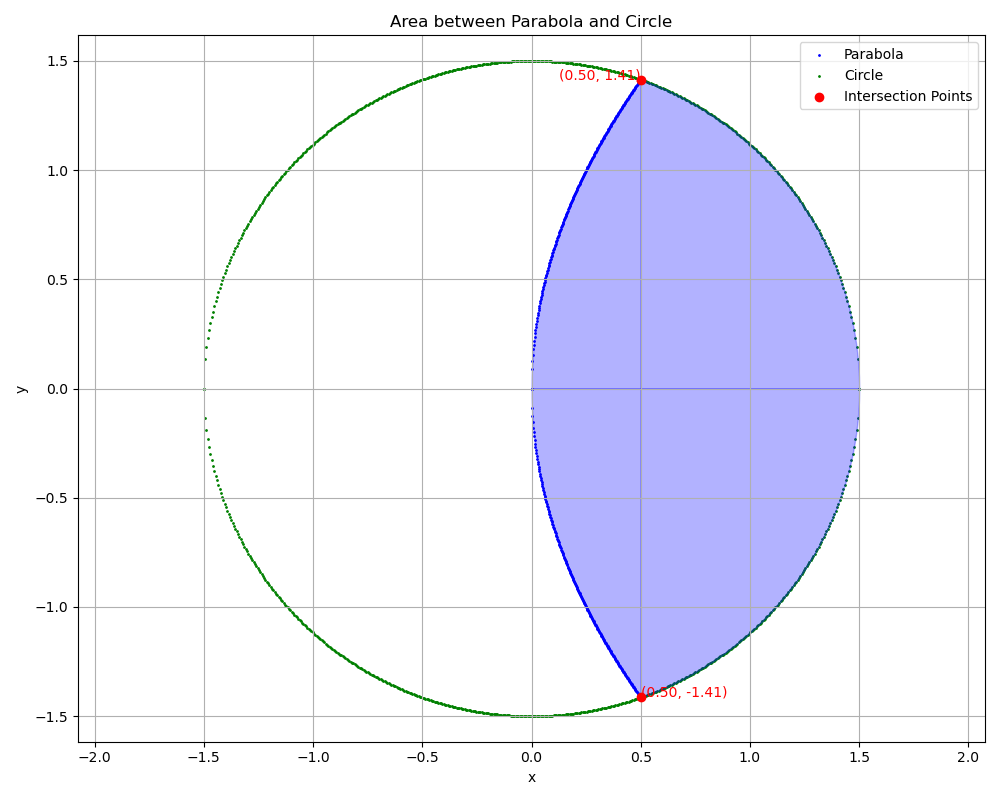
\includegraphics[width=0.7\linewidth]{figs/area.png}
	\caption{Area between Circle and Parabola}
   \end{figure}
\end{document}

